
C++ classes are often “empty,” which means that their internal representation does not require any bits of memory at run time. This is the case typically for classes that contain only type members, nonvirtual function members, and static data members. Nonstatic data members, virtual functions, and virtual base classes, on the other hand, do require some memory at running time.

Even empty classes, however, have nonzero size. Try the following program if you’d like to verify this:

\hspace*{\fill} \\ %插入空行
\noindent
\textit{inherit/empty.cpp}
\begin{lstlisting}[style=styleCXX]
#include <iostream>

class EmptyClass {
};

int main()
{
	std::cout << "sizeof(EmptyClass): " << sizeof(EmptyClass) << ’\n’;
}
\end{lstlisting}

For many platforms, this program will print 1 as size of EmptyClass. A few systems impose more strict alignment requirements on class types and may print another small integer (typically, 4).

\subsubsubsection{21.1.1\hspace{0.2cm}Layout Principles}

The designers of C++ had various reasons to avoid zero-size classes. For example, an array of zerosize classes would presumably have size zero too, but then the usual properties of pointer arithmetic would no longer apply. For example, let’s assume ZeroSizedT is a zero-size type:

\begin{lstlisting}[style=styleCXX]
ZeroSizedT z[10];
...
&z[i] - &z[j] // compute distance between pointers/addresses
\end{lstlisting}

Normally, the difference in the previous example is obtained by dividing the number of bytes between the two addresses by the size of the type to which it is pointing, but when that size is zero this is clearly not satisfactory.

However, even though there are no zero-size types in C++, the C++ standard does specify that when an empty class is used as a base class, no space needs to be allocated for it provided that it does not cause it to be allocated to the same address as another object or subobject of the same type. Let’s look at some examples to clarify what this empty base class optimization (EBCO) means in practice. Consider the following program:

\hspace*{\fill} \\ %插入空行
\noindent
\textit{inherit/ebco1.cpp}
\begin{lstlisting}[style=styleCXX]
#include <iostream>

class Empty {
	using Int = int; // type alias members don’t make a class nonempty
};

class EmptyToo : public Empty {
};

class EmptyThree : public EmptyToo {
};

int main()
{
	std::cout << "sizeof(Empty): " << sizeof(Empty) << ’\n’;
	std::cout << "sizeof(EmptyToo): " << sizeof(EmptyToo) << ’\n’;
	std::cout << "sizeof(EmptyThree): " << sizeof(EmptyThree) << ’\n’;
}
\end{lstlisting}

If your compiler implements the EBCO, it will print the same size for every class, but none of these classes has size zero (see Figure 21.1). This means that within class EmptyToo, the class Empty is not given any space. Note also that an empty class with optimized empty bases (and no other bases)  is also empty. This explains why class EmptyThree can also have the same size as class Empty. If your compiler does not implement the EBCO, it will print different sizes (see Figure 21.2).

\begin{center}
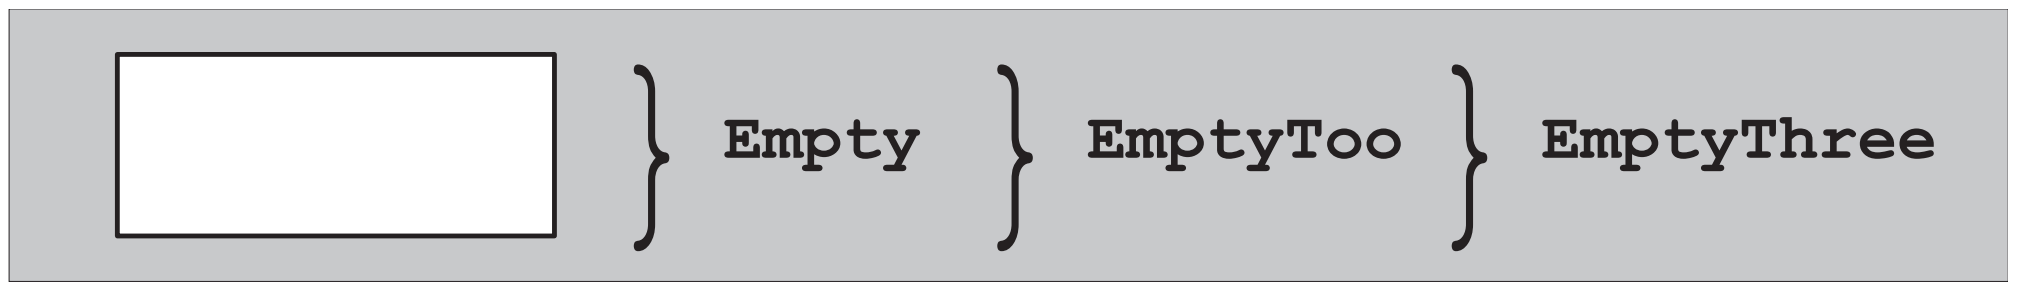
\includegraphics[width=0.8\textwidth]{content/3/chapter21/images/1.png} \\
Figure 21.1. Layout of EmptyThree by a compiler that implements the EBCO
\end{center}

\begin{center}
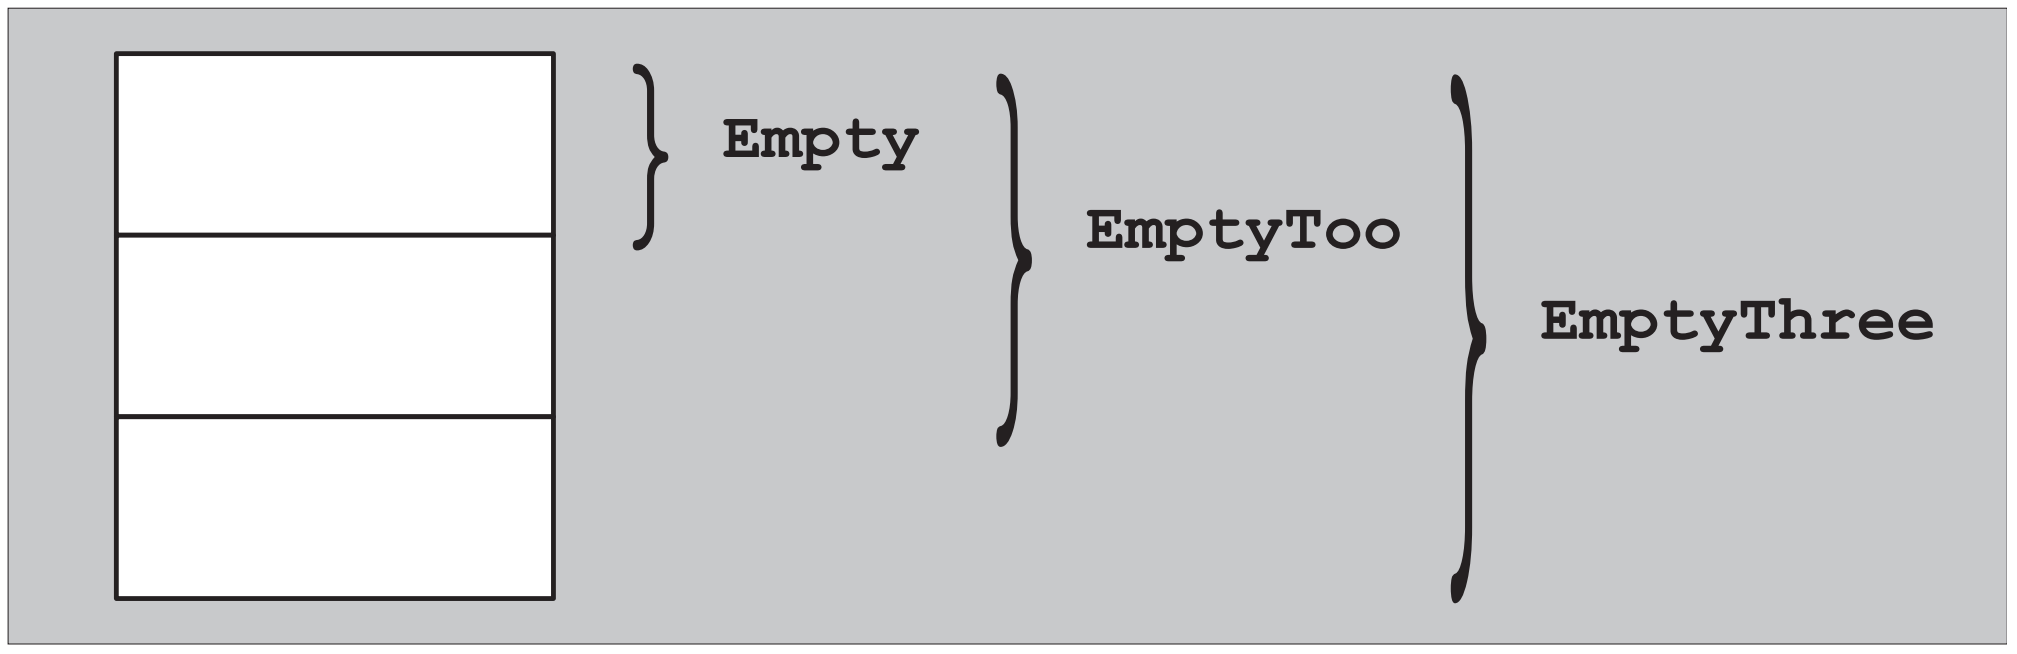
\includegraphics[width=0.8\textwidth]{content/3/chapter21/images/2.png} \\
Figure 21.2. Layout of EmptyThree by a compiler that does not implement the EBCO
\end{center}

Consider an example that runs into a constraint of the EBCO:

\hspace*{\fill} \\ %插入空行
\noindent
\textit{inherit/ebco2.cpp}
\begin{lstlisting}[style=styleCXX]
#include <iostream>

class Empty {
	using Int = int; // type alias members don’t make a class nonempty
};

class EmptyToo : public Empty {
};

class NonEmpty : public Empty, public EmptyToo {
};

int main()
{
	std::cout << "sizeof(Empty): " << sizeof(Empty) << ’\n’;
	std::cout << "sizeof(EmptyToo): " << sizeof(EmptyToo) << ’\n’;
	std::cout << "sizeof(NonEmpty): " << sizeof(NonEmpty) << ’\n’;
}
\end{lstlisting}

It may come as a surprise that class NonEmpty is not an empty class. After all, it does not have any members and neither do its base classes. However, the base classes Empty and EmptyToo of NonEmpty cannot be allocated to the same address because this would cause the base class Empty of EmptyToo to end up at the same address as the base class Empty of class NonEmpty. In other words, two subobjects of the same type would end up at the same offset, and this is not permitted by the object layout rules of C++. It may be conceivable to decide that one of the Empty base subobjects is placed at offset “0 bytes” and the other at offset “1 byte,” but the complete NonEmpty object still cannot have a size of 1 byte because in an array of two NonEmpty objects, an Empty subobject of the first element cannot end up at the same address as an Empty subobject of the second element (see Figure 21.3).

\begin{center}
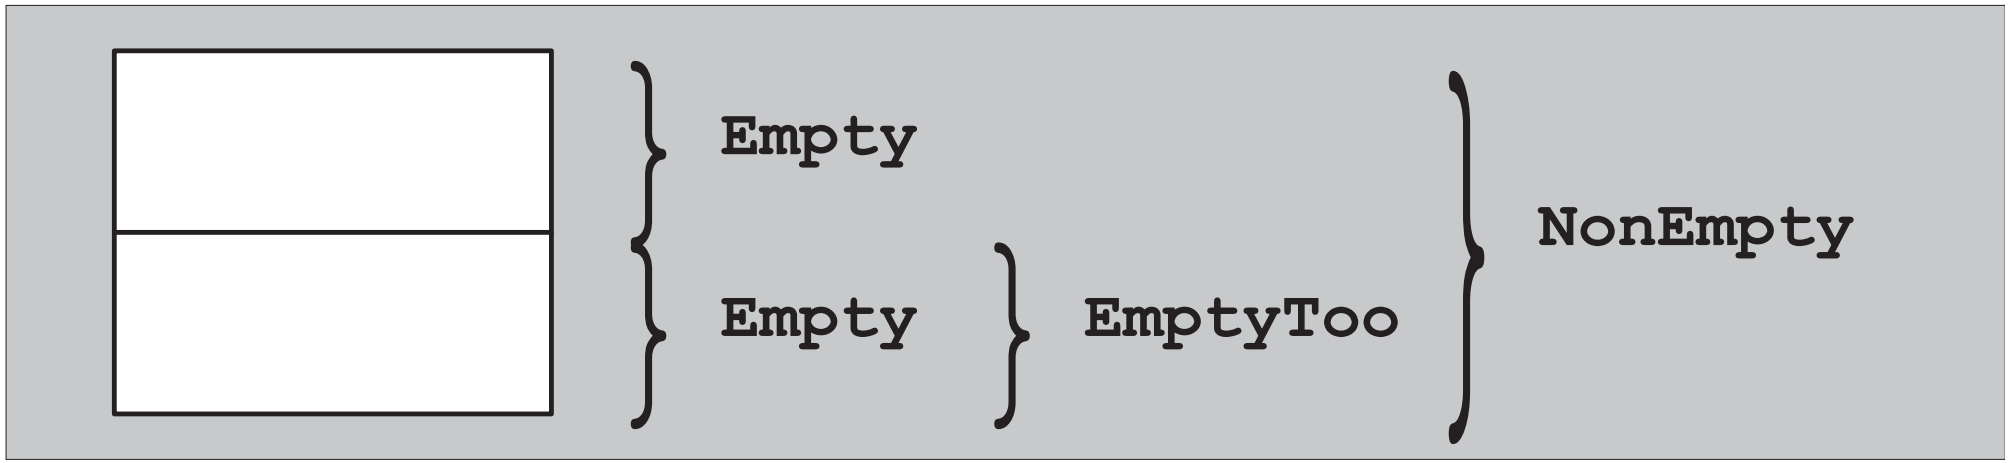
\includegraphics[width=0.8\textwidth]{content/3/chapter21/images/3.png} \\
Figure 21.3. Layout of NonEmpty by a compiler that implements the EBCO
\end{center}

The rationale for the constraint on the EBCO stems from the fact that it is desirable to be able to compare whether two pointers point to the same object. Because pointers are nearly always internally represented as just addresses, we must ensure that two different addresses (i.e., pointer values) correspond to two different objects.

The constraint may not seem very significant. However, in practice, it is often encountered because many classes tend to inherit from a small set of empty classes that define some common type aliases. When two subobjects of such classes are used in the same complete object, the optimization is inhibited.

Even with this constraint, the EBCO is an important optimization for template libraries because a number of techniques rely on the introduction of base classes simply for the purpose of introducing new type aliases or providing extra functionality without adding new data. Several such techniques will be described in this chapter.

\subsubsubsection{21.1.2\hspace{0.2cm}Members as Base Classes}

The EBCO has no equivalent for data members because (among other things) it would create some problems with the representation of pointers to members. As a result, it is sometimes desirable to implement as a (private) base class what would at first sight be thought of as a member variable. However, this is not without its challenges.

The problem is most interesting in the context of templates because template parameters are often substituted with empty class types, but in general we cannot rely on this rule. If nothing is known about a template type parameter, the EBCO cannot easily be exploited. Indeed, consider the following trivial example:

\begin{lstlisting}[style=styleCXX]
template<typename T1, typename T2>
class MyClass {
	private:
	T1 a;
	T2 b;
	...
};
\end{lstlisting}

It is entirely possible that one or both template parameters are substituted by an empty class type. If this is the case, then the representation of MyClass<T1,T2> may be suboptimal and may waste a word of memory for every instance of a MyClass<T1,T2>.

This can be avoided by making the template arguments base classes instead:

\begin{lstlisting}[style=styleCXX]
template<typename T1, typename T2>
class MyClass : private T1, private T2 {
};
\end{lstlisting}

However, this straightforward alternative has its own set of problems:

\begin{itemize}
\item 
It doesn’t work when T1 or T2 is substituted with a nonclass type or with a union type.

\item 
It also doesn’t work when the two parameters are substituted with the same type (although this can be addressed fairly easily by adding another layer of inheritance; see page 513).

\item 
The class may be final, in which case attempts to inherit from it will cause an error.
\end{itemize}

Even if we satisfactorily addressed these problems, a very serious problem persists: Adding a base class can fundamentally modify the interface of the given class. For our MyClass class, this may not seem significant because there are very few interface elements to affect, but as we see later in this chapter, inheriting from a template parameter can affect whether a member function is virtual. Clearly, this approach to exploiting the EBCO is fraught with all kinds of trouble.

A more practical tool can be devised for the common case when a template parameter is known to be substituted by class types only and when another member of the class template is available. The main idea is to “merge” the potentially empty type parameter with the other member using the EBCO. For example, instead of writing

\begin{lstlisting}[style=styleCXX]
template<typename CustomClass>
class Optimizable {
	private:
	CustomClass info; // might be empty
	void* storage;
	...
};
\end{lstlisting}

a template implementer would use the following:

\begin{lstlisting}[style=styleCXX]
template<typename CustomClass>
class Optimizable {
	private:
	BaseMemberPair<CustomClass, void*> info_and_storage;
	...
};
\end{lstlisting}

Even without seeing the implementation of the template BaseMemberPair, it is clear that its use makes the implementation of Optimizable more verbose. However, various template library implementers have reported that the performance gains (for the clients of their libraries) do justify the added complexity. We explore this idiom further in our discussion of tuple storage in Section 25.1.1 on page 576.

The implementation of BaseMemberPair can be fairly compact:

\hspace*{\fill} \\ %插入空行
\noindent
\textit{inherit/basememberpair.hpp}
\begin{lstlisting}[style=styleCXX]
#ifndef BASE_MEMBER_PAIR_HPP
#define BASE_MEMBER_PAIR_HPP

template<typename Base, typename Member>
class BaseMemberPair : private Base {
	private:
	Member mem;
	
	public:
	// constructor
	BaseMemberPair (Base const & b, Member const & m)
	: Base(b), mem(m) {
	}
	// access base class data via first()
	Base const& base() const {
		return static_cast<Base const&>(*this);
	}
	Base& base() {
		return static_cast<Base&>(*this);
	}
	// access member data via second()
	Member const& member() const {
		return this->mem;
	}
	Member& member() {
		return this->mem;
	}
};

#endif // BASE_MEMBER_PAIR_HPP
\end{lstlisting}

An implementation needs to use the member functions base() and member() to access the encapsulated (and possibly storage-optimized) data members.





























